\section{Implementierung des YARN"=Modells}
\label{sec:yarnModel}

Das implementierte YARN"=Modell besteht, wie bereits in \cref{sec:modelArchitecture} gezeigt, aus fünf Komponenten und den Komponentenfehlern der hier relevanten YARN"=Komponenten.
Die vier implementierten YARN"=Komponenten sind die Anwendungen, ihre Attempts und Container, sowie die Nodes.
Zudem wurde eine Klasse implementiert, die zur Repräsentation des \gls{RM} und als Controller zum Testen mit \gls{ss} dient.
Einen Überblick über den Aufbau des implementierten YARN"=Modells gibt das in \cref{fig:yarnModelClassDiagram} dargestellte Klassendiagramm.

\begin{figure}
    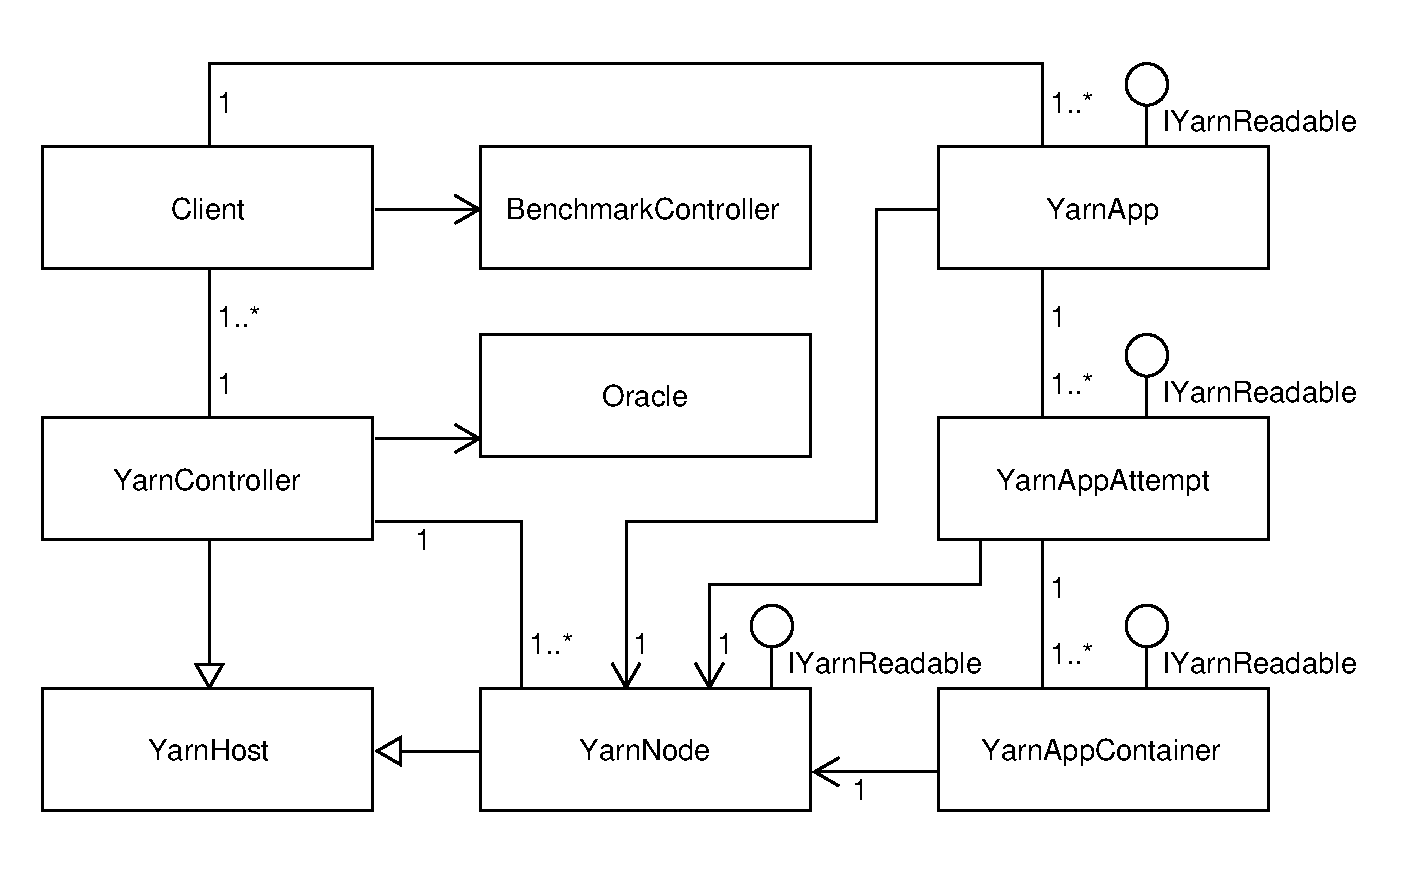
\includegraphics{./resources/yarnModel_ls_MA.pdf}
    \caption[Grundlegender Aufbau des YARN"=Modells]
        {Grundlegender Aufbau des YARN"=Modells.
        Assoziationen und weitere Verbindungen zum Treiber und \acrshort{ss} sind hier aus Gründen der Übersichtlichkeit nicht dargestellt.}
    \label{fig:yarnModelClassDiagram}
\end{figure}

Im Klassendiagramm wird zudem ersichtlich, dass jedem Client mehrere Anwendungen in Form der Klasse \texttt{YarnApp} zugeordnet sind, jeder Anwendung mehrere Attempts (\texttt{YarnAppAttempt}) und jedem Attempt mehrere YARN"=Container (\texttt{YarnAppContainer}).
Der Client stellt somit auch die den relevanten YARN"=Komponenten übergeordnete Komponente dar.

Zunächst wird im Folgenden die dem Modell übergeordnete zentrale Klasse \texttt{Model} erläutert, danach die relevanten YARN"=Komponenten mit ihren Komponentenfehlern, anschließend die anderen Komponenten des YARN"=Modells.
Der Aufbau des Benchmark"=Controllers wird in \cref{sec:benchmarkController} erläutert.

\subsection{Die Klassen Model und ModelSettings}
\label{subsec:modelClass}

Die Klasse \texttt{Model} stellt die zentrale Schnittstelle des Testsystems mit \gls{ss} dar (vgl. \cref{subsec:ssharpModel}), während die Klasse \texttt{ModelSettings} generelle, variable Einstellungen und Konstanten für das Testsystem bereitstellt.
Da die \texttt{Model}"=Klasse auch das gesamte Modell repräsentiert, wird sie zur Verwaltung des von \gls{ss} auszuführenden Modells genutzt.
Hierfür werden alle Komponenten, wie Clients oder Anwendungen, zusätzlich zur Struktur innerhalb des Modells auch in \texttt{Model} gespeichert, welche zur Interaktion mit \gls{ss} entsprechenden Attributen versehen sind (vgl. \cref{subsec:ssharpModel}).

Daneben dient die Klasse auch zur Initialisierung des gesamten Modells.
Hierbei werden zunächst der Controller, der Treiber in Form der benötigten Parser und Connectoren, sowie die Nodes des Clusters initialisiert.
Anschließend wird für jeden Client eine gewisse Anzahl an \texttt{YarnApp}"=Instanzen zum Speichern der Daten von Anwendungen, für jede Anwendung eine gewisse Anzahl an \texttt{YarnAppAttempt}"=Instanzen für Attempts, sowie für jeden Attempt eine gewisse Anzahl an \texttt{YarnAppContainer} für die Daten der YARN"=Container initialisiert.
Die genaue Anzahl der erzeugten Instanzen kann hierbei für jede YARN"=Komponente und auch für Clients nach Bedarf angepasst werden, wodurch auch einzelne Komponenten, wie \zB in der Fallstudie die YARN"=Container, deaktiviert werden können.

Alle initialisierten YARN"=Komponenten werden durch die \texttt{Model}"=Klasse auch innerhalb des Modells zur Verfügung gestellt, sofern Komponenten diese benötigen.
Darunter zählen auch die bei der Ausführung des Modells benötigten Parser und Connectoren des Treibers.
Aufgrund der Einschränkungen von \gls{ss} im Umgang mit dem Treiber (vgl. \cref{subsec:driverModelIntegration}) sowie zur einfacheren Bereitstellung von benötigten Komponenten und Funktionen im Modell, ist die \texttt{Model}"=Klasse als Singleton realisiert.

Die \texttt{ModelSettings}"=Klasse dient zum Speichern der variablen Einstellungen sowie zum Bereitstellen von generellen Konstanten für das Modell bzw. Testsystem.
Gespeichert und bereitgestellt werden hier Daten, wie \zB die Zugangsdaten der SSH"=Verbindungen oder der genutzte \texttt{HostMode} (vgl.  \cref{subsec:implementedConnectors,subsec:hostMode}).
Die \texttt{ModelSettings}"=Klasse ist dabei zur Verwaltung des \texttt{HostMode}s zuständig und dafür verantwortlich, die vom \texttt{HostMode} abhängigen Pfade und Adressen dem Treiber bereit zu stellen.
Dies betrifft \zB den Pfad zum benötigten Setup"=Script (vgl. \cref{subsec:scripts}) oder die zur Nutzung der REST"=API benötigten Adressen.
Eine Besonderheit bildet hierbei die Eigenschaft \texttt{HttpUrl} der \texttt{YarnNode}s, welche beim Initialisieren des Modells durch die \texttt{ModelSettings} die zum \texttt{HostMode} passende Adresse erhält (vgl. \cref{subsec:yarnComponents,subsec:hostMode}).

\subsection{Relevante YARN"=Komponenten}
\label{subsec:yarnComponents}

Die vier implementierten, relevanten YARN"=Komponenten sind die Anwendungen, ihre Attempts und Container sowie die Nodes des Clusters.
Diese vier implementierten YARN"=Komponenten stellen das zum Testen mit \gls{ss} benötigte Modell des \gls{SuT} dar (vgl. \cref{subsec:ssharpModel}).
Obwohl die YARN"=Container in dieser Fallstudie nicht benötigt werden, waren sie für die Fallstudie \cite{Eberhardinger2018} notwendig, welche ebenfalls mit dem hier beschriebenen Modell durchgeführt wurde.

Eine Übersicht über die Implementierung der für diese Fallstudie relevanten YARN"=Komponenten gibt folgendes Klassendiagramm:

\begin{figure}[h]
    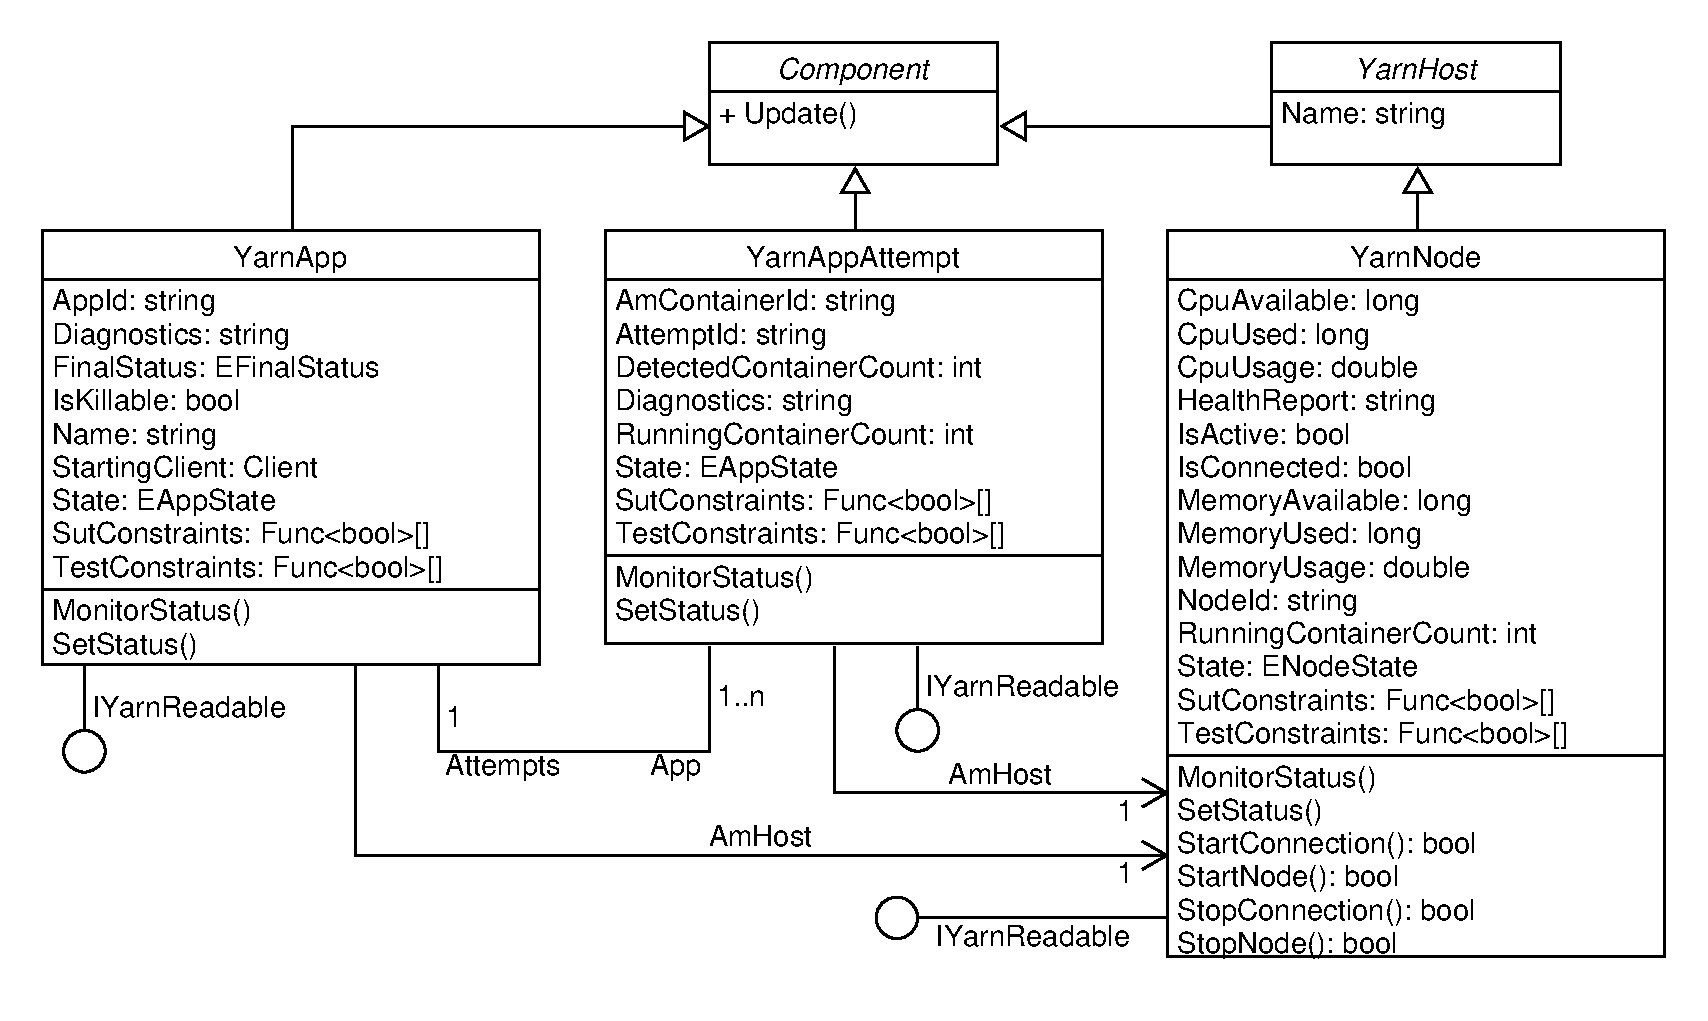
\includegraphics[width=\columnwidth]{./resources/yarnComponents.pdf}
    \caption[Für die Fallstudie relevante, implementierte YARN"=Komponenten]
        {Für die Fallstudie relevante, implementierte YARN"=Komponenten, hier dargestellt mit den wichtigsten Eigenschaften und Methoden.
        Dies sind alle für die spätere Durchführung und zur Ausgabe des Zustandes (vgl. \cref{subsec:dataOrganisation}) wichtigen Eigenschaften und Methoden.
        Aus Gründen der Übersichtlichkeit sind die implementierten Komponentenfehler, einige der \texttt{IYarnReadable} bereitgestellten, relevanten Eigenschaften und Methoden sowie die Klasse \texttt{YarnAppContainer} nicht aufgeführt.}
    \label{fig:yarnComponentsClassDiagram}
\end{figure}

Die Eigenschaft \texttt{AmHost} speichert den ausführenden Node des \gls{AppMstr} der Anwendung bzw. des Attempts, die Eigenschaft \texttt{IsKillable} gibt an, ob eine Anwendung derzeit ausgeführt wird und somit vorzeitig abgebrochen werden kann.
Die Eigenschaften \texttt{Diagnostics} bzw. \texttt{HealthReport} stellen von Hadoop zur Verfügung gestellte, weitere Diagnostik"=Informationen bei Fehlern dar.
Die \texttt{State}"=Eigenschaften bzw. \texttt{FinalState} speichern die von Hadoop angegebenen Zustände der YARN"=Komponenten.
Hierfür wurden entsprechende Enumerationen, basierend auf den in \cite{HadoopRmApi271} angegebenen möglichen Werten, für die jeweiligen Zustände im Modell implementiert.

Da für diese Fallstudie die Daten der Container selbst nicht relevant sind, wird im hier verwendeten Modell nur gespeichert, wie viele YARN"=Container beim Monitoring im aktuellen Testfall (\texttt{RunningContainerCount}) bzw. für alle bisher ausgeführten Testfälle kumuliert (\texttt{DetectedContainerCount}) erkannt wurden.
Für die Tests \cite{Eberhardinger2018} werden die Daten der Container genauso wie die der anderen YARN"=Komponenten gespeichert.
Hierfür enthalten die Klassen \texttt{YarnAppAttempt} und \texttt{YarnAppContainer} entsprechende Eigenschaften zur jeweiligen Zuordnung, analog zu denen zwischen \texttt{YarnApp} und \texttt{YarnAppAttempt}.
Analoge Zuordnungen bestehen auch zu den Clients bzw. den YARN"=Containern, sofern benötigt.
Die Eigenschaft \texttt{AmContainerId} speichert zudem die Container"=ID des \gls{AppMstr}"=Containers.

Die Eigenschaften mit den Präfixen \texttt{CPU} bzw. \texttt{Memory} in \texttt{YarnNode} dienen zur Speicherung der derzeitigen Auslastung der CPU"=Kerne bzw. des Speichers eines Nodes.
Benötigt werden diese Werte zur Berechnung, ob ein Komponentenfehler aktiviert oder deaktiviert wird (vgl. \cref{subsec:faultActivation}).
Die durch die Basisklasse \texttt{YarnHost} bereitgestellte Eigenschaft \texttt{HttpUrl} beschreibt die für die Nutzung der REST"=API benötigte Adresse des Nodes (vgl. \cref{subsubsec:implRestConnector}).
Da die Adresse vom \texttt{HostMode} abhängig ist, wird sie mithilfe der \texttt{ModelSettings} beim initialisieren des Modells entsprechend festgelegt (vgl. \cref{subsec:hostMode,subsec:modelClass}).

Die Eigenschaften \texttt{SutConstraints} und \texttt{TestConstraints} sowie die Methoden \texttt{MonitorStatus()} und \texttt{SetStatus()} werden von \texttt{IYarnReadable} bereitgestellt und speichern die Constraints bzw. dienen zur Durchführung des Monitorings der implementierten Komponenten (vgl. \cref{subsec:yarnComponentInterface}).
Die Start"= und Stop"=Methoden sowie die Eigenschaften \texttt{IsActive} und \texttt{IsConnected} in \texttt{YarnNode} dienen zur Identifikation und Injektion bzw. Reparatur der Komponentenfehler (vgl. \cref{subsec:yarnComponentFaults}).

Neben den dargestellten, relevanten Eigenschaften und Methoden wurden zahlreiche weitere implementiert, welche einerseits zur Vollständigkeit der implementierten Komponenten für die Tests \cite{Eberhardinger2018}, andererseits auch zur Ausführung mithilfe des \gls{ss}"=Frameworks benötigt werden.
Letztere sind \zB zur Speicherung von Strings notwendig, welche aufgrund der Einschränkungen von \gls{ss} (vgl. \cref{sec:ssharp}) \uU nicht jederzeit frei genutzt werden können.
Strings sind im YARN"=Modell daher zur Speicherung immer als  \texttt{char}"=Arrays implementiert, werden jedoch zur einfacheren Nutzung im Modell in Strings konvertiert:

\begin{lstlisting}[label=lst:modelCharArrayAsString,style=cs,
caption={[Implementierung der Eigenschaft AppId]
    Implementierung der Eigenschaft \texttt{AppId}.
    Die beiden Methoden \texttt{GetCharArrayAsString} und \texttt{SetCharArrayOnString} führen die Konvertierung in den \texttt{char}"=Array bzw. des \texttt{char}"=Arrays in einen String durch.
    Das Attribut \texttt{NonSerializable} definiert, dass die Eigenschaft bei der Ausführung der Simulation von \acrshort{ss} ignoriert wird.}]
public char[] AppIdActual { get; }

[NonSerializable]
public string AppId
{
  get { return ModelUtilities.GetCharArrayAsString(AppIdActual); }
  set { ModelUtilities.SetCharArrayOnString(AppIdActual, value); }
}
\end{lstlisting}

Die \texttt{Update()}"=Methoden starten bei allen vier implementierten YARN"=Komponenten die jeweiligen Monitoring"=Funktionen, bei \texttt{YarnNode} werden zudem \texttt{StartNode()} und \texttt{StartConnection()} ausgeführt um mögliche zuvor injizierte Komponentenfehler im realen Cluster zu reparieren.

Da bei der Ausführung des Modells durch \gls{ss} keine neuen Instanzen erzeugt werden können (vgl. \cref{sec:ssharp}), dienen die jeweiligen IDs der Komponenten auch als Indikator, ob die jeweilige Komponenten"=Instanz derzeit benötigt wird und somit Daten gespeichert werden sollen.
Daher wird das Monitoring auch nur dann ausgeführt, wenn der Instanz eine nicht leere ID, \zB in Form der \texttt{AppId}, zugewiesen wurde.

\subsection{Implementierung der Komponentenfehler}
\label{subsec:yarnComponentFaults}

Die im YARN"=Modell implementierten Komponentenfehler wurden direkt in den entsprechenden YARN"=Komponenten implementiert.
Implementiert wurden hierbei mit \texttt{NodeDeadFault} und \texttt{NodeConnectionErrorFault} zwei jeweils als \texttt{TransientFault} definierte Komponentenfehler für die durch \texttt{YarnNode} repräsentierten Nodes.
Während durch \texttt{NodeDeadFault} der komplette Node beendet wird, trennt \texttt{NodeConnectionErrorFault} nur die Verbindung des Nodes zum Cluster.
Die dazugehörigen Effekt"=Klassen der Komponentenfehler sind jeweils als innere Klassen in \texttt{YarnNode} implementiert.

Die Injizierung und Reparatur der beiden Fehler geschieht mithilfe der vier Stop- bzw. Start"=Methoden, wie \zB \texttt{StopNode()}, die bereits im Klassendiagramm in \cref{fig:yarnComponentsClassDiagram} zu sehen sind.
Wenn ein Komponentenfehler aktiviert wird, wird durch die Effekt"=Klasse die jeweilige Stop"=Methode ausgeführt und so der Fehler injiziert:

\begin{lstlisting}[label=lst:faultInjection,,style=cs,
caption={[Injizierung des Komponentenfehlers NodeDeadFault]
    Injizierung des Komponentenfehlers \texttt{NodeDeadFault} (gekürzt).
    Sollte der Node nicht beendet werden, wird die Injizierung einmalig erneut versucht.
    \texttt{CmdConnector.Faulting} stellt die zur Injizierung verwendete SSH"=Verbindung dar.}]
public class YarnNode : YarnHost, IYarnReadable
{
  [NodeFault]
  public readonly Fault NodeDeadFault = new TransientFault();
  public IHadoopConnector FaultConnector { get; set; }
  
  public bool StopNode(bool retry = true)
  {
    if(IsActive)
    {
      var isStopped = FaultConnector.StopNode(Name);
      if(isStopped)
        IsActive = false;
      else if(retry)
        StopNode(false); // t§§ry again once
    }
    return !IsActive;
  }
  
  [FaultEffect(Fault = nameof(NodeDeadFault))]
  public class NodeDeadEffect : YarnNode
  {
    public override void Update()
    {
      StopNode();
    }
  }
}

public class CmdConnector : IHadoopConnector
{
  private SshConnection Faulting { get; }
  
  public bool StopNode(string nodeName)
  {
    var id = DriverUtilities.ParseInt(nodeName);
    Faulting.Run($"{Model.HadoopSetupScript} hadoop stop {id}",
       IsConsoleOut);
    return !CheckNodeRunning(id);
  }
}
\end{lstlisting}

Die Reparatur von Komponentenfehlern geschieht analog hierzu.
Hierfür werden in der \texttt{Update()}"=Methode die beiden Start"=Methoden aufgerufen, um einen defekten Node zu reparieren.
Eine Besonderheit bildet hierbei die Reparatur des Komponentenfehlers \texttt{NodeConnectionErrorFault}, welche den Node komplett neu startet, da sich der Node ansonsten möglicherweise nicht wieder mit dem \gls{RM} verbinden kann.

Da beide Fehler zudem auch gleichzeitig aktiviert werden können, wurde dem Komponentenfehler \texttt{NodeDeadFault} mithilfe entsprechender \gls{ss}"=Funktionen eine höhere Priorität vergeben, wodurch dieser Vorrang vor dem anderen Komponentenfehler erhält.
Dadurch wird in solchen Fällen der Node beendet und nicht zunächst noch zusätzlich auch vom Netzwerk getrennt.

Zur einfachen Identifikation der aktiven Komponentenfehler innerhalb des YARN"=Modells dienen die beiden Eigenschaften \texttt{IsActive} und \texttt{IsConnected}.
In \cref{lst:faultInjection} wird bereits die Auswirkung der beiden Eigenschaften gezeigt, indem verhindert wird, dass ein möglicherweise bereits injizierter bzw. reparierter Komponentenfehler erneut injiziert bzw. repariert wird.
Sie dienen aber auch zur Validierung der Constraints, bei denen mithilfe der beiden Eigenschaften geprüft wird, ob ein Node korrekt als aktiv bzw. defekt erkannt wurde.

\subsection{Aktivierung von Komponentenfehlern}
\label{subsec:faultActivation}

Die Aktivierung von Komponentenfehlern ist von folgenden Parametern abhängig:

\begin{itemize}
    \item Auslastung des Nodes im vorhergehenden Testfall
    \item Generelle Wahrscheinlichkeit zur Fehleraktivierung
    \item Einer Zufallszahl
\end{itemize}

Der hierfür benötigte Zufallsgenerator wird mithilfe des spezifizierten Basisseeds initialisiert (vgl. \cref{subsec:testcaseGeneration}).
Da der Zufallsgenerator ein statischer Generator ist, werden über einen Test bei der gleichen Anzahl an möglichen Komponentenfehlern immer die gleichen Werte zurückgegeben, nicht jedoch zwingend für einen bestimmten Komponentenfehler eines Nodes.
Die Entscheidung zur Aktivierung bzw. Injizierung der Komponentenfehler wird somit auch nicht automatisiert durch \gls{ss} durchgeführt, sondern mithilfe von speziell hierfür entwickelten Klassen und Methoden (vgl. \cref{subsec:ssharpExecution}).

Um bei der Ausführung eines Testfalls bestimmen zu können, ob ein Komponentenfehler aktiviert wird, sind alle Komponentenfehler mit dem Attribut \texttt{NodeFault} markiert.
Dieses Attribut enthält die notwendigen Berechnungen, um über die Aktivierung des Komponentenfehlers zu entscheiden:

\begin{lstlisting}[label=lst:faultActivationCalc,style=cs,
caption={[Berechnung der Aktivierung von Komponentenfehlern]
    Berechnung der Aktivierung von Komponentenfehlern (zusammengefasst).}]
var node = AllNodes.First(n => n.Name == nodeName);
var nodeUsage = (node.MemoryUsage + node.CpuUsage) / 2;

if(nodeUsage < 0.1) nodeUsage = 0.1;
else if(nodeUsage > 0.9) nodeUsage = 0.9;

NodeUsageOnActivation = nodeUsage; // f§§or u§§sing on repairing

var faultUsage = nodeUsage * ActivationProbability * 2;

var probability = 1 - faultUsage;
var randomValue = RandomGen.NextDouble();
Logger.Info($"Activation probability: {probability} < {randomValue}");
return probability < randomValue;
\end{lstlisting}

Die Entscheidung zur Deaktivierung eines Komponentenfehlers verhält sich analog.
Anstatt der generellen Aktivierungswahrscheinlichkeit wird hierbei die generelle Wahrscheinlichkeit zur Deaktivierung der Komponentenfehler genutzt.
Außerdem spielt bei der Deaktivierung die Auslastung des Nodes zum Zeitpunkt der Aktivierung eine Rolle, welche hierzu in der Eigenschaft \texttt{NodeUsageOnActivation} des Attributs entsprechend gespeichert und zur Deaktivierung genutzt wird.
Zudem wird ein Komponentenfehler eher deaktiviert, wenn der Node eine geringe Auslastung aufweist, während die Aktivierung bevorzugt bei einer hohen Auslastung durchgeführt wird.

\subsection{Interface IYarnReadable und Monitoring}
\label{subsec:yarnComponentInterface}

Das Interface \texttt{IYarnReadable} ist das zentrale Erkennungsmerkmal der im Modell abgebildeten und implementierten YARN"=Komponenten.
Es dient zum einen zur Identifikation aller implementierten YARN"=Komponenten, andererseits stellt es auch Eigenschaften und Methoden bereit, welche einerseits dem Testen mit \gls{ss} dienen, primär aber dem Ermitteln der Daten aus dem realen Cluster:

\begin{itemize}
    \item \texttt{GetId()}
    \item \texttt{StatusAsString()}
    
    \item \texttt{Parser}
    \item \texttt{IsSelfMonitoring}
    \item \texttt{MonitorStatus()}
    \item \texttt{SetStatus()}
    
    \item \texttt{PreviousParsedComponent}
    \item \texttt{CurrentParsedComponent}
    \item \texttt{SutConstraints}
    \item \texttt{TestConstraints}
\end{itemize}

Die beiden erstgenannten Methoden dienen primär zu Debugging"=Zwecken und zur Rückgabe der ID beim Zugriff auf die jeweiligen Komponenten mithilfe das Interfaces bzw. der Werte aller Eigenschaften der Komponente als ein String.

Die nachfolgenden vier Eigenschaften und Methoden dienen zum Monitoring der entsprechenden YARN"=Komponenten.
Während die Eigenschaft \texttt{Parser} den zu verwendenden Parser (vgl. \cref{subsec:implementedParsers}) speichert, dient die Eigenschaft \texttt{IsSelfMonito""ring} zur Unterscheidung, ob die Daten einer Komponente von dieser selbst ermittelt werden oder dies die übergeordnete Komponente durchführt.
Diese Unterscheidung ist nötig, da YARN hierfür zwei unterschiedliche Schnittstellen bietet: Die Rückgabe der Daten durch die \gls{CLI} oder mithilfe der REST"=API.
Bei der Nutzung der \gls{CLI} zur Ermittlung der Daten eignet sich die Selbstermittlung der Daten besser, während bei der Nutzung der REST"=API die Ermittlung der Daten durch die übergeordnete Komponente geeigneter ist; die Gründe hierfür sind in \cref{subsubsec:implRestParser} erläutert.
Daher ist auch die Methode \texttt{SetStatus()} definiert, da hier unabhängig von der Datenermittlung der aktuelle Status der Komponente abgespeichert werden kann.
Die Durchführung des Monitoring findet in beiden Fällen mithilfe der Methode \texttt{MonitorStatus()} statt:

\begin{lstlisting}[label=lst:monitorAppStatus,style=cs,
caption={[Implementierung der Methode MonitorStatus() in der Klasse YarnApp]
    Implementierung der Methode \texttt{MonitorStatus()} in der Klasse \texttt{YarnApp} (gekürzt).
    Das Monitoring der anderen Komponenten erfolgt analog hierzu.}]
public void MonitorStatus()
{
  if(IsSelfMonitoring)
  {
    var parsed = Parser.ParseAppDetails(AppId);
    if(parsed != null)
    SetStatus(parsed);
  }
  
  var parsedAttempts = Parser.ParseAppAttemptList(AppId);
  foreach(var parsed in parsedAttempts)
  {
    // search attempt with t§§his id or an free attempt
    attempt.IsSelfMonitoring = IsSelfMonitoring;
    if(IsSelfMonitoring)
      attempt.AttemptId = parsed.AttemptId;
    else
    {
      attempt.SetStatus(parsed);
      attempt.MonitorStatus();
    }
  }
}
\end{lstlisting}

Beim Monitoring der untergeordneten Komponenten wird zunächst immer geprüft, ob bereits eine Instanz mit der ID der Komponente vorhanden ist.
Wenn dies der Fall ist, werden die vom realen Cluster ermittelten Daten weiterhin in der bereits bestehenden Instanz gespeichert, ansonsten wird eine freie Instanz genutzt, um die Daten der Subkomponente zu speichern.
Wenn keine freie Instanz mehr vorhanden ist, wird eine entsprechende \texttt{OutOfMemoryException} ausgelöst, damit die Ausführung des Modells abgebrochen werden kann.

Eine Besonderheit bildet das Monitoring der YARN"=Container.
Da eine Anwendung sehr schnell eine sehr hohe Anzahl an Containern allokiert und jede Container"=Instanz im Modell Speicherplatz benötigt, werden nur die Daten der während des Monitoring ausgeführten Container ermittelt.
Bei Anwendungen und Attempts werden dagegen auch die Daten von bereits beendeten Anwendungen bzw. Attempts gespeichert.

Die vier restlichen Eigenschaften und Methoden des Interfaces dienen zur Auswertung der Komponente durch \gls{ss}.
Die beiden Eigenschaften \texttt{SutConstraints} und \texttt{TestConstraints} dienen zur Implementierung der in \cref{sec:requirements} definierten Anforderungen in Form von Constraints.

\subsection{Constraints der YARN"=Komponenten}
\label{subsec:yarnComponentConstraints}

Die meisten der in \cref{sec:requirements} definierten Anforderungen an das \gls{SuT} und gesamte Testsystem sind auch für die YARN"=Komponenten relevant und werden in Form von Constraints im Modell implementiert (vgl. \cref{subsec:ssharpModel,sec:clusterSetup,sec:requirements}).
Die relevanten Bestandteile der Anforderungen für die jeweiligen Komponenten sind mithilfe der beiden in \texttt{IYarnReadable} definierten Eigenschaften \texttt{SutConstraints} und \texttt{TestConstraints} implementiert.
Realisiert sind die beiden Eigenschaften für die Constraints jeweils als \texttt{Func<bool>[]}:

\begin{lstlisting}[label=lst:constraintDefinition,style=cs,
caption={[Definition der Constraints in YarnApp]
    Definition der Constraints in \texttt{YarnApp} (gekürzt)}]
public Func<bool>[] SutConstraints => new Func<bool>[]
{
  // task will be completed i§§f not canceled
  () =>
  {
    if(FinalStatus != EFinalStatus.FAILED)
      return true;
    if(!String.IsNullOrWhiteSpace(Name) &&
        Name.ToLower().Contains("fail job"))
      return true;
    return false;
  },
  // configuration will be updated
};

public Func<bool>[] TestConstraints => new Func<bool>[]
{
  // current state i§§s detected and saved
  () =>
  {
    var prev = PreviousParsedComponent as IApplicationResult;
    var curr = CurrentParsedComponent as IApplicationResult;
    // compare prev, curr and t§§his and r§§eturn the result
    // or otherwise
    return false;
  },
};
\end{lstlisting}

Die Constraints werden im Anschluss an das Monitoring vom Oracle validiert (vgl. \cref{subsec:oracleImpl}).
Die Constraints sind so definiert, dass im Falle einer erfolgreichen Validierung \texttt{true} zurückgegeben wird, in allen anderen Fällen die Rückgabe \texttt{false} dagegen eine nicht erfolgreiche Validierung anzeigt.

Wenn die ID der Komponenten"=Instanzen leer ist, und die jeweilige Instanz somit derzeit nicht im Modell zum Speichern der Daten des realen Clusters benötigt wird, werden die Constraints immer erfolgreich validiert.

\subsection{Implementierung des Clients}
\label{subsec:yarnClient}

Der Client im YARN"=Modell simuliert einen Client und dient somit zum Starten der Benchmarks.
Die Auswahl des zu startenden Benchmarks erfolgt durch den Benchmark"=Controller, welcher in \cref{sec:benchmarkController} erläutert wird.
Jeder Client besitzt hierzu einen eigenen Benchmark"=Controller, womit die auszuführenden Benchmarks für jeden Client unabhängig von anderen Clients ausgewählt werden.
Ein Client kann jedoch nur eine Anwendung gleichzeitig starten und muss eine zuvor gestartete Anwendung beenden, bevor er eine neue starten kann.
Dies wird jedoch nur durchgeführt, wenn sich der auszuführende Benchmark geändert hat:

\begin{lstlisting}[label=lst:startClientBenchmark,style=cs,
caption={[Auswahl und Start des nachfolgenden Benchmarks]
    Auswahl und Start des nachfolgenden Benchmarks (gekürzt).
    Die Methode \texttt{ChangeBenchmark()} des Benchmark"=Controllers wird in \cref{subsec:selectionNextBenchmark} erläutert.}]
public void UpdateBenchmark()
{
  var benchChanged = BenchController.ChangeBenchmark();
  
  if(benchChanged)
  {
    StopCurrentBenchmark();
    StartBenchmark(BenchController.CurrentBenchmark);
  }
}

public void StartBenchmark(Benchmark benchmark)
{
  if(benchmark.HasOutputDir)
    SubmittingConnector.RemoveHdfsDir(
       benchmark.GetOutputDir(ClientDir));
  var appId = SubmittingConnector.StartApplicationAsyncTillId
     (benchmark.GetStartCmd(ClientDir));
  // save application id
}
\end{lstlisting}

Da die auf dem Cluster ausgeführten Anwendungen \uU nicht gestartet werden, wenn im HDFS das Ausgabeverzeichnis bereits vorhanden ist, muss dieses beim Starten eines Benchmarks zunächst gelöscht werden.
Um mehrere Clients unabhängig voneinander nutzen zu können, besitzt jeder Client zudem ein spezifisches Verzeichnis, das seiner eigenen Client"=ID entspricht.
Die Ein- und Ausgabedaten werden dadurch nur im Verzeichnis des jeweiligen Clients gespeichert.

Wenn eine Anwendung gestartet wurde, wird diese zunächst synchron ausgeführt, bis von der gestarteten Anwendung ihre vom Cluster zugewiesene Anwendungs"=ID zurückgegeben wird.
Diese ID wird vom Client abgespeichert und wird dafür benötigt, um in späteren Testfällen die Anwendung wieder beenden zu können.
Zudem wird auch eine noch leere \texttt{YarnApp}"=Instanz ermittelt und dieser die ID ebenfalls zugewiesen, um diese analog zu den anderen YARN"=Komponenten zum Speichern der Daten der Anwendung zu nutzen.
Der Unterschied zu anderen Komponenten ist jedoch, dass immer eine neue Instanz genutzt wird, da eine neue Anwendung in der Regel eine im Cluster noch nicht vorhandene ID erhält.
Wenn keine leere \texttt{YarnApp}"=Instanz mehr verfügbar ist, wird analog zum Monitoring ebenfalls eine \texttt{OutOfMemoryException} ausgelöst.

\subsection{Implementierung des Controllers}
\label{subsec:yarnController}

Der Controller repräsentiert den \gls{RM} des Hadoop"=Clusters, weshalb er genauso wie die modellierten Nodes von \texttt{YarnHost} erbt.
Primär dient er jedoch als Controller zum Testen mit \gls{ss} (vgl. \cref{subsec:ssharpModel}).
Er steuert daher den wesentlichen Ablauf eines Testfalls und ist die einzige Komponente des YARN"=Modells, die direkt mit dem Oracle interagiert:

\begin{lstlisting}[label=lst:controllerUpdate,style=cs,
caption={[Update()"=Methode des Controllers]
    \texttt{Update()}"=Methode des Controllers (gekürzt).
    Eine ausführliche Beschreibung des gesamten Ablaufs eines Testfalls findet sich in \cref{subsec:simulationStep}.}]
public override void Update()
{
  MonitorMarp();
  
  foreach(var client in ConnectedClients)
    client.UpdateBenchmark();
  
  // optional, to allocate at least the AM container
  ModelUtilities.Sleep(5);
  
  MonitorAll();
  
  Oracle.ValidateConstraints(EConstraintType.Sut);
  Oracle.IsReconfPossible();
  Oracle.ValidateConstraints(EConstraintType.Test);
}
\end{lstlisting}

Nach einem ersten Monitoring des \gls{MARP}"=Wertes wird durch den Controller sichergestellt, dass jeder simulierte Client eine Anwendung startet, sofern vom Benchmark"=Controller hierbei eine neue Anwendung ausgewählt wird (vgl. \cref{subsec:yarnClient,sec:benchmarkController}).

Vor dem Monitoring wird zunächst fünf Sekunden gewartet, damit die gestarteten Anwendungen auf dem Cluster die benötigten Ressourcen erhalten können, wodurch die Auslastung des Clusters besser ermittelt werden kann.
Zum Monitoring nutzt der Controller die von \texttt{IYarnReadable} bereitgestellte Eigenschaft, um das Selbstmonitoring der einzelnen YARN"=Komponenten zu deaktivieren und führt dabei das Monitoring der Nodes und Anwendungen aus.
Er startet zudem bei jeder Anwendung auch das Monitoring der jeweiligen Attempts bzw. dadurch auch das der YARN"=Container, sofern benötigt.
Dabei wird der \gls{MARP}"=Wert hier erneut ausgelesen, da er sich abhängig von den ausgeführten Anwendungen jederzeit verändern kann.
Abschließend startet der Controller die Validierung der Constraints durch das Oracle, getrennt nach Constraints für das \gls{SuT} und das gesamte Testsystem, sowie die Prüfung, ob eine weitere Rekonfiguration des Clusters möglich ist.

Für den Controller selbst sind ebenfalls einige der in \cref{sec:requirements} definierten Anforderungen relevant.
Die hierbei relevanten Anforderungen sind ebenfalls direkt im Controller implementiert und werden durch das Oracle validiert.

\subsection{Implementierung des Oracles}
\label{subsec:oracleImpl}

Das Oracle dient zur automatisierten Validierung der in \cref{sec:requirements} definierten Anforderungen durch das Testsystem (vgl. \cref{subsec:ssharpModel}).
Hierzu werden die Constraints aller YARN"=Komponenten und des Controllers validiert und geprüft, ob eine Rekonfiguration des Clusters möglich ist.
Da die beiden von \texttt{IYarnReadable} bereitgestellten Eigenschaften zum Speichern der Constraints vom Typ \texttt{Func<bool>[]} sind, können so jeweils alle implementierten Constraints nacheinander validiert werden:

\begin{lstlisting}[label=lst:oracleValidateConstraints,style=cs,
caption={[Validieren der Constraints durch das Oracle]
    Validieren der Constraints durch das Oracle.
    Die zu validierenden Constraints werden im Parameter \texttt{constraints} übergeben, der Parameter \texttt{constraintType} dient zu statistischen Zwecken in \texttt{CountCheck()}.}]
public static bool ValidateConstraints(string componentId,
   Func<bool>[] constraints, EConstraintType constraintType)
{
  var isCompontenValid = true;
  for(var i = 0; i < constraints.Length; i++)
  {
    var constraint = constraints[i];
    bool isValid;
    try
    {
      isValid = constraint();
    }
    catch
    {
      isValid = false;
    }
    
    CountCheck(constraintType, isValid);
    if(!isValid)
    {
      Logger.Error($"YARN component not valid: " +
         "Constraint {i} in {componentId}");
      if(isCompontenValid)
        isCompontenValid = false;
    }
  }
  
  return isCompontenValid;
}
\end{lstlisting}

Bei der Prüfung, ob eine weitere Rekonfiguration möglich ist, wird geprüft, ob alle Nodes im Cluster defekt sind bzw. dies beim Monitoring des realen Clusters erkannt wurde.
Wenn dies der Fall ist, wird die weitere Testausführung gemäß \cref{subsec:testRequirements} abgebrochen, indem eine \texttt{Exception} ausgelöst wird:

\begin{lstlisting}[label=lst:oracleIsReconfPossible,style=cs,
caption={Prüfung nach der Möglichkeit weiterer Rekonfigurationen}]
public bool IsReconfPossible()
{
  var isReconfPossible = ConnectedNodes
     .Any(n => n.State == ENodeState.RUNNING);
  if(!isReconfPossible)
  {
    Logger.Error("No reconfiguration possible!");
    throw new Exception("No reconfiguration possible!");
  }
  return true;
}
\end{lstlisting}

Die bereits in \cref{lst:oracleValidateConstraints} gezeigte Methode \texttt{CountCheck()} dient zu statistischen Zwecken.
Hierbei wird getrennt nach Constraint"=Typ (der funktionalen Anforderungen an das \gls{SuT} oder aller Anforderungen an das Testsystem) gezählt, wie viele Constraints insgesamt validiert, und wie viele davon verletzt wurden.
Die jeweiligen Werte können beim Abschluss einer Testausführung entsprechend ausgegeben werden.
